\documentclass{article}

\usepackage{graphicx}
\usepackage{amsmath}
\graphicspath{ {./images/} }

\usepackage[greek,english]{babel}
\usepackage{alphabeta}



\title{Άσκηση 1}
\author{Χρήστος Αλέξανδρος Τσιγγιρόπουλος}
\date{29 December 2021}



\begin{document}
    \maketitle
    \section{Σύγκριση Επαναλήψεων}
    
    Το αποτέλεσμα του προγράμματος είναι:
    
Μέθοδος Διχοτόμησης :

Διάστημα [0.0, 1.5]

Η ρίζα είναι : 0.8571424484  και χρειάστηκαν 19  επαναλήψεις

Διάστημα [1.5, 3.0]

Η ρίζα είναι : 1.9921875000  και χρειάστηκαν 6  επαναλήψεις

Newton - Raphson    :

Διάστημα [0.0, 1.5]

Η ρίζα είναι : 0.8571428347  και χρειάστηκαν 6  επαναλήψεις

Διάστημα [1.5, 3.0]

Η ρίζα είναι : 1.9913170896  και χρειάστηκαν 9  επαναλήψεις

Μέθοδος Τέμνουσας   :

Διάστημα [0.0, 1.1]

Η ρίζα είναι : 0.8571435319  και χρειάστηκαν 9  επαναλήψεις

Διάστημα [1.1, 3.0]

Η ρίζα είναι : 2.0109433844  και χρειάστηκαν 13  επαναλήψεις
    \section{Σχόλια Αποτελέσματος}
    
    Παρατηρούμε ότι η μέθοδος Newton-Raphson είναι η πίο γρήγορη στο παράδειγμα μας απο την Μέθοδο Διχοτόμησης για την εύρεση της ίδιας ρίζας (0.8571...) ακόμα και απο την μέθοδο της τέμνουσας που υλοποιείτε σε πιο μικρό διάστημα. 
    Για την δεύτερη ρίζα δεν ισχύει όμως το αντίστοιχο αφού η μέθοδος Διχοτόμησης καταλήγει πιο γρήγορα απο τις άλλες 2 με την μέθοδο Newton-Raphson να χρειάζεται λίγες περισσότερες επαναλλήψεις.
    Συμπερασματικά, κατά μέσο όρο στο παράδειγμα μας η μέθοδος Newton-Raphson είναι η πίο γρήγορη με 7,5 επαναλήψεις ανα ρίζα.
    Δεύτερη είναι η μέθοδος Τέμνουσας με 10,5 επαναλήψεις ανα ρίζα 
    και στο τέλος η μέθοδος διχοτόμησης με 12,5 επαναλήψεις ανά ρίζα.
    \section{ Τετραγωνική σύγκλιση στη μέθοδο Newton - Raphson}
    
    Για να συγκλίνει η μέθοδος αυτή τετραγωνικά σε μία ρίζα, θα πρέπει η ρίζα αυτή, να μην είναι πολλαπλότητας μεγαλύτερης ή ίσης του δύο. Ακόμα και τότε όμως θα συγκλινει. Και απο ότι έχω καταλάβει θα ήταν καλύτερο να μην υπήρχε κάποιο σημείο y στο διάστημα που να έκανε την f'(y)=0 
    γιατί τότε το κλάσμα:    
    \begin{equation}
        |\frac{f(x)}{f'(x)}|>>0
    \end{equation} θα γινόταν αρκετά μεγάλος αριθμός κοντά στο ξ και έτσι το χ με δείκτη n+1 θα απομακρινόταν αρκετά απο το χ με δείκτη n
    \section{ Περιγραφή Κώδικα}
    
    Υπάρχουν 3 συναρτήσεις  για τις 3 μεθόδους που η κάθε μία παίρνει σαν όρισμα την αρχή και το τέλος του διαστήματος δλδ στο παράδειγμα μας το x=0,y=1.5 και x=1.5,y=3 : 
    \begin{itemize}
    \item {dixotomisi(x,y)}
    
    Η συνάρτηση αυτή υλοποιεί την διχοτόμηση.
    Για το μέσο mid=(x+y)/2 ελέγχουμε αρχικά αν είναι ρίζα της εξίσωσης και αν ναι τότε την τυπώνει μαζί με τις επαναλήψεις που χρειάστηκαν για να βρεθεί και επιστρέφει, 
    στην σνέχεια βρήσκουμε το νέο διάστημα ελέγχοντας αν το 
    \begin{equation}
       f(x)f(mid)<0
    \end{equation}
    και αν ναι τότε το y = mid 
    αλλιώς αν το 
    \begin{equation}
       f(y)*f(mid) <0
    \end{equation} και αν ναι τότε το y = mid και το νέό διάστημα είναι το (x,y) δλδ βρήσκουμε για ποιο διάστημα ισχύει το θεώρημα Bolzano.
    Επαναλαμβάνουμε την ίδια διαδικασία μέχρι να βρεθεί μια προσεγγιση της ρίζας.
    
    \item newton-raphson(x,y)
    
    Παρόμοια χρησιμοποιώ μια μεταβλητή 
    \begin{equation}
       x_n = x_{n-1} - \frac{f(x_{n-1})}{f'(x_{n-1})}
    \end{equation}
    αποθηκεύω το xn στο x και ελέγχω αν xn είναι ρίζα της εξίσωσης αν ναι τότε την τυπώνει μαζί με τις επαναλήψεις που χρειάστηκαν για να βρεθεί και η συνάρτηση επιστρέφει.
    Επαναλαμβάνουμε την ίδια διαδικασία μέχρι να βρεθεί μια προσεγγιση της ρίζας.
    
    \item temnousa(x,y)
    
    Παρόμοια και για την μέθοδο της τέμνουσας έχω: 
    \begin{equation}
        x_{n+1} = x_n - \frac{f(x_n)(x_n - x_{n-1})}{f(x+n) - f(x_{n-1})}
    \end{equation}
    αποθηκεύω το xn+1 στο xn και το xn στο xn-1 και ελέγχω αν το xn είναι ρίζα της εξίσωσης αν ναι τότε την τυπώνει μαζί με τις επαναλήψεις που χρειάστηκαν για να βρεθεί και η συνάρτηση επιστρέφει.
    
    \item{Βοηθητικές συναρτήσεις}
    
    Επιπλέον υπάρχουν οι συναρτήσεις 
    f(x),f1(x),f2(x) 
    που επιστρέφουν τις 
    f(x),f'(x),f''(x) αντίστοιχα.
\end{itemize}


\begin{figure}[h]
\section{Γραφική παράσταση}
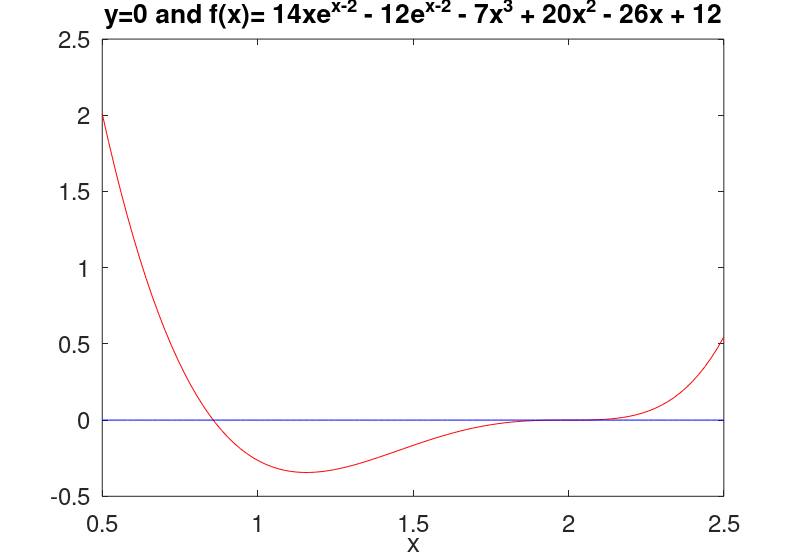
\includegraphics[width=12cm]{one.png}
\end{figure}

\end{document}